\begin{figure*}[hbt]
\centering
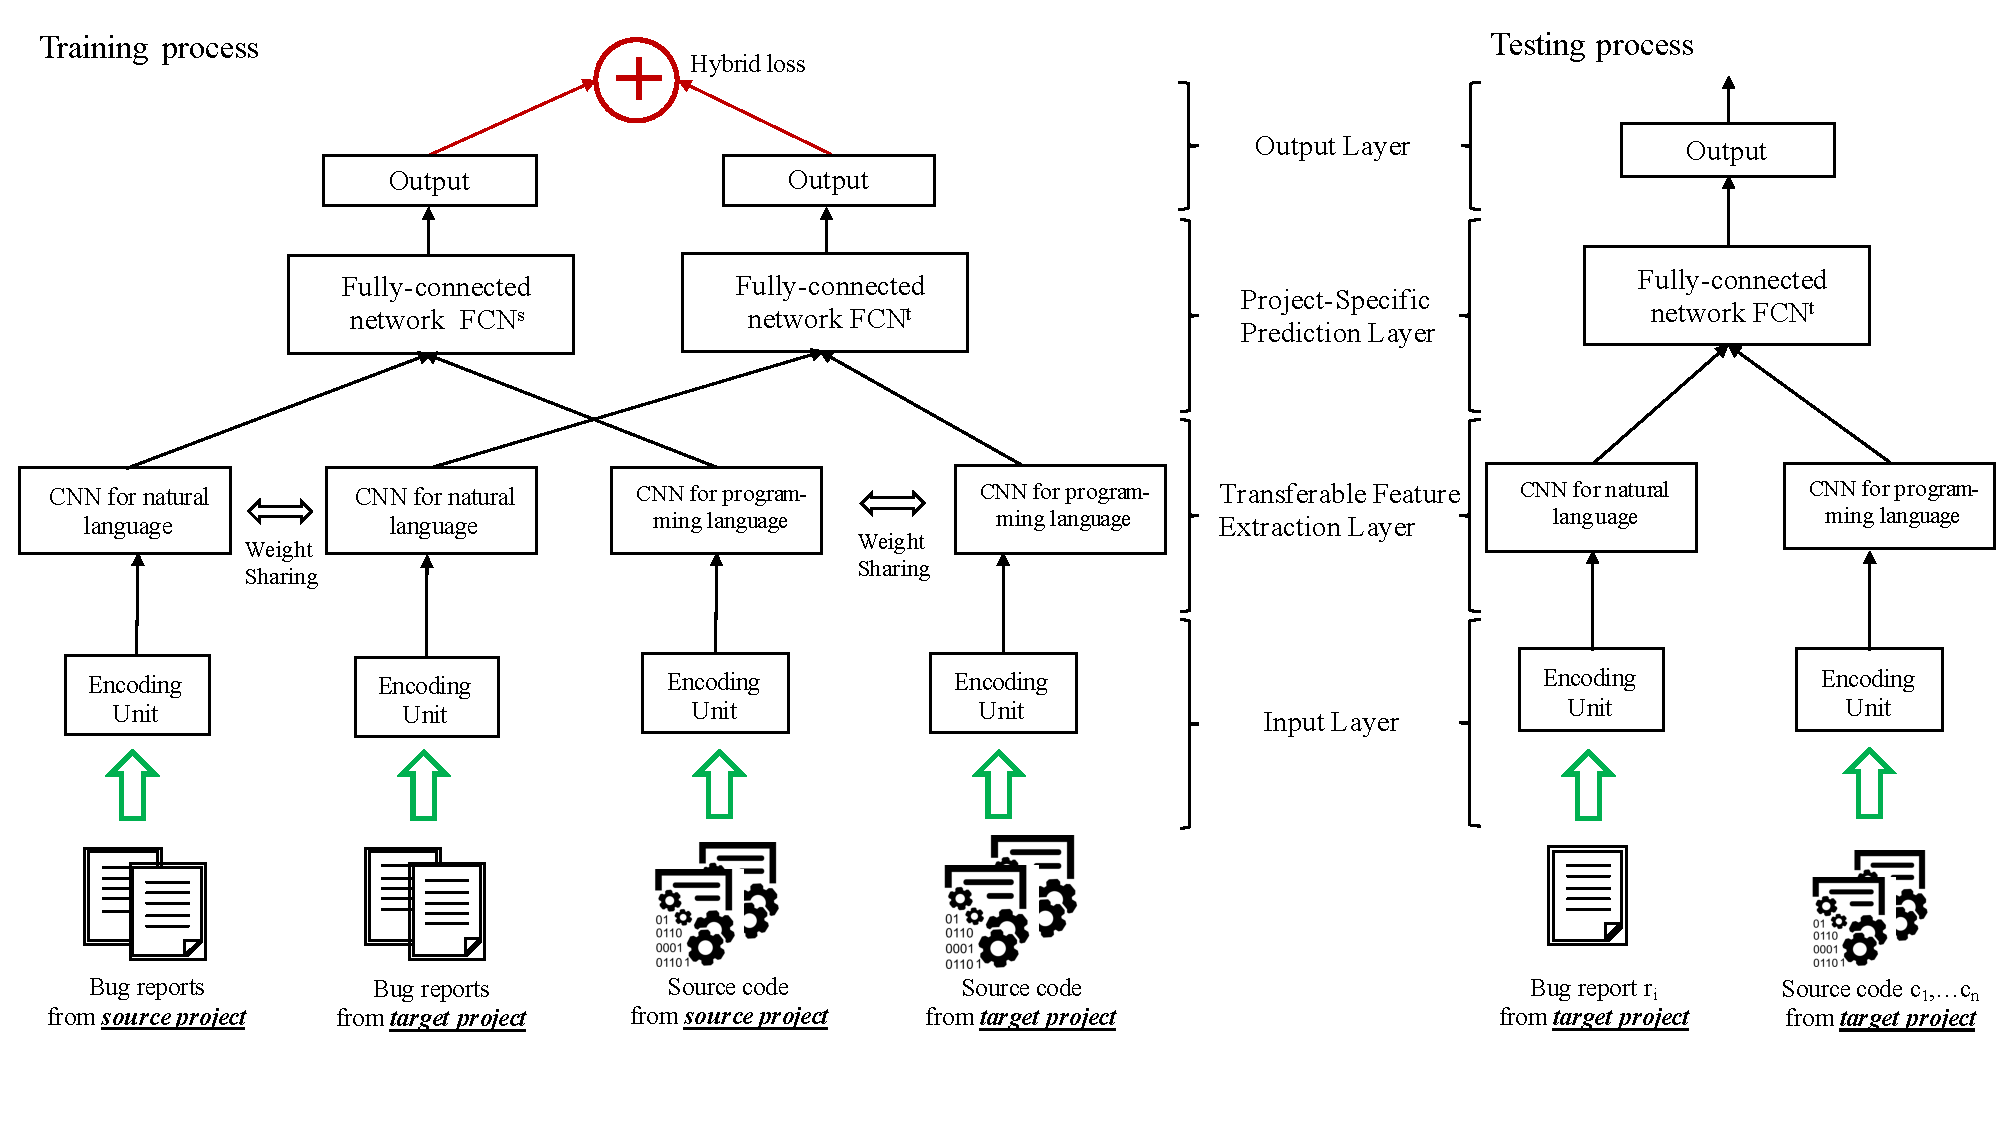
\includegraphics[width = 2\columnwidth]{pic/structure.pdf}
\caption{The overall structure of Transfer Natural and Programming language CNN.  The left part is the training process of \TRANPCNN based on the bug reports and source code from source projects and a few data from target projects, the weights of which are trained by minimizing the loss of ensemble loss from fully-connected networks $fc_s$ and $fc_t$. The right part is the testing process, a new bug report and its candidate source code are fed into the model, and \TRANPCNN outputs their relevant scores for bug localization.}
\label{fig:structure}
\end{figure*}

In cross-project bug localization, we are provided with a \emph{source} project with many bug reports carefully localized to the corresponding source code and a \emph{target} project in which only several bug reports are localized. The goal is to construct a model to fully leverage the rich information from the source project to facilitate the bug localization for the target project. 

Let $\mathcal{C}^s =   \{ { c^s_1, c^s_2}, \cdots, c^s_{n^c_1} \} $ and $\mathcal{C}^t =\{ c^t_1, c^t_2, \cdots, c^t_{n^c_2} \}$ denote the set of source codes from the source project and the target project, respectively, and $\mathcal{C}=\mathcal{C}^s \bigcup \mathcal{C}^t $. Let $\mathcal{R}^s =\{ r^s_1, r^s_2, \cdots, r^s_{n^r_1}\}$ and $\mathcal{R}^t =\{ r^t_1, r^t_2, \cdots, r^t_{n^r_2}\}$ denote the bug reports related to the source project and target project, respectively, $\mathcal{R}=\mathcal{R}^s \bigcup \mathcal{R}^t $, where $n^c_1, n^c_2, n^r_1, n^r_2$ denote the number of source files and bug reports from source project and target project, respectively. We formulate cross-project bug localization as a learning task which aims to learn prediction functions $\mathbf{f}=(f^s,f^t), f^\alpha: \mathcal{R}^\alpha \times \mathcal{C}^\alpha \mapsto \mathcal{Y}^\alpha$. $y^\alpha_{ij} \in \mathcal{Y}^\alpha = \{+1, -1\}$ indicates whether a source code $c^\alpha_j \in \mathcal{C}^\alpha $ is relevant to a bug report $r^\alpha_i \in \mathcal{R}^\alpha$, $\alpha \in (s,t)$. 

Since the source project and the target project may differ from each other in the way how a bug report is localized to the corresponding source code, to effectively learn the prediction function for the target project, one problem should be addressed carefully, i.e., how to identify the information that potentially useful for learning the prediction function. Intuitively, if the information from the source project can be used for the target project, they must share something internal in common; the reason making them different is the shared internal commonalities works in different ways. Therefore, we argue that the model that facilitate an effective cross-project bug localization can be constructed by 1) learning shared internal feature representations from both source and target project, and 2) biasing the learner towards project-specific properties based on the shared internal feature representations. 

We instantiate the aforementioned idea by proposing a novel deep transfer neural network named \TRANPCNN (TRAnsfer Natural and Program Language Convolutional Neural Network), Firstly, \TRANPCNN takes bug reports and source codes as inputs and learns the common transferable feature representation shared by both source and target project, and then elaborates to biasing the prediction functions towards the source and target project, respectively, based on the shared feature representation, in order to generate project-specific predictions for the target domain.


\subsection{Model Structure}
The model structure of \TRANPCNN is depicted in Figure~\ref{fig:structure}, where the subfigure to the left depicts the training process of \TRANPCNN, while subfigure to the right depicts the corresponding test process. 

\TRANPCNN consists four parts: the input layer, the transferable feature extraction layers, project-specific correlation fitting layers and the output layer. The input layer takes the bug report as well as the source code in its original format and generate their corresponding encodings such that they can be further processed by the subsequent layers of \TRANPCNN; the transferable feature extraction layers aim to learn the intermediate feature representations from the bug reports and source codes, respectively, such that the common knowledge shared by both the source project and the target project which can eventually facilitate the identification of the correlation between the bug report and the source codes; the project-specific prediction layer is responsible for biasing the learning based on the transferable feature representation towards the project-specific correlation patterns between the bug reports and source codes in source project and target project, respectively; the output layers generate the final correlation scores for the report-code pairs based on the fitted correlations in the source domain and the target domain, respectively. It is obvious that the the transferable feature extraction layers and project-specific correlation fitting layers are the key parts of the proposed model, which would be explained in details in the following subsections.

To train this model, report-code pairs from the source project and target project along with their ground truth correlation labels are fed into the proposed deep model in order to learn the transferable feature representation shared by both source and target projects as well as the project-specific prediction functions for the source and target project, respectively. After the model is fully trained, prediction function $f^{t}$ would be used for determine the correlation of the report-code pair $(r_i^t, c_j^t)$ from the target project.

\subsection{Transferable Feature Extraction Layer}
When provided with the bug report and codes from the source and target project in their original format, the encodings for the bug reports and the source codes are first generated by the preceded input layer. Traditional TFIDF representation fails to capture correlation between terms. Thus, we employ word2vec encoding to represent both the bug reports and the source codes in the purpose of enriching the initial representation, based on which, the transferable features are further extracted.

The transferable features for bug report and the source codes should satisfy the following properties. First, the transferable features should be able to represent the functional semantics in both bug reports and source codes such that the semantics can be further utilized to identify the correlation patterns between the reports and the codes. Second, the extract semantics should be able to embed some common knowledge between the source project and target project such that those knowledge learned from the source project can be eventually transferred to facilitate the learning for the target project.

To make the embedded knowledge to be transferable between source and target projects, the key challenge here is how to identify what information is useful and transferable and what is useful but may not be transferred to other projects. To address this challenge, we employ a special strategy called \emph{weight sharing} during the learning process, which imposes a hard constraint that the learned weights in the network (either N-CNN or P-CNN) for the target project should be exactly the same as the the learned weights in the network for the source project. By weight sharing, the learning procedure that facilitates good performance on both source project and target project is forced to focus on those common features shared by both source project and target project rather than extracting the project-specific features for each project. Thus, the resulting features eventually \emph{transfer} the common knowledge that are useful for determine the correlation between the bug report and the source code from the source project to the target project. Note that such knowledge may need a large amount of labeled training data to be learned for any single project, but now can be directly used for the target project where the labeled training data may be limited especially for the code start. 

\subsection{Project-specific Correlation Fitting Layers}
After the transferable feature extraction layers, the bug reports (as well as the source codes) from both source and target project are represented using the \emph{same} set of transferable features embedded with common knowledge shared by both source and target project. However, since the source project and target project differ in how the bug reports and the source codes are correlated, the subsequent project-specific correlation fitting layers are employed to fit the model to capture the project-specific correlation patterns based on the same set of transferable features.

The key challenge here is how to learn prediction functions with different goals (i.e., to perform well in the source and target projects, respectively) based on the same set of features within the same model structure. To address this challenge, we construct two fully connected neural network substructures, namely $fc^s$ and $fc^t$, for the subsequent project-specific correlation fitting layers, where $fc^s$ and $fc^t$ share the same input unit and have different output unit. Such a special design facilitate the model to take the same set of transferable features from both bug report and source code and fit to correlation pattern of the report-code pair in the source project and target project, respectively, with different substructures $fc^s$ and $fc^t$.

In order to fit the two network substructures $fc^s$ and $fc^t$ to different correlation patterns within the same model structure, we propose a hybrid loss function (Eq. \ref{eq:lossfunction}) to unify the loss from different goals into the one loss function.
\begin{equation}
\begin{aligned}
\label{eq:lossfunction}
\mathop{\arg\min}_{\mathbf{W}}&\sum_{s_i,s_j}\mathcal{L}(\mathbf{h}_{s_i},\mathbf{h}_{s_j}
,y_{s_{ij}}; W_{fc_s}, W_{conv} ))\\
+&\sum_{t_i,t_j}\mathcal{L}(\mathbf{h}_{t_i},\mathbf{h}_{t_j},y_{t_{ij}}; W_{fc_t}, W_{conv})+\lambda||\mathbf{W}||^2
\end{aligned}
\end{equation}
where, $\mathcal{L}$ is the square loss, $\lambda$ is the trade-off parameter and the weight vectors $W$ contains the weight vectors in convolutional neural networks $W_{conv}$, in fully-connected network of source domain $W_{fc_s}$ and in fully-connected network of target domain $W_{fc_t}$.

By solving this optimization problem using the stochastic gradient descent (SGD), the proposed \TRANPCNN can be effectively learned.
